\subsection{Prototypical Networks for Small Datasets}
\label{models:protonet}

Prototypical Networks \cite{protonet} is a meta-learning model for the problem of few-shot classification, where a classifier must generalize to new classes not seen in the training set, given only a small number of examples of each new class. The ability of a algorithm to perform few-shot learning is typically measured by its performance on n-shot, k-way classification tasks. First a model is given a query sample belonging to a new, previously unseen class. Then, it’s also given a support set, S, consisting of n examples, each from k different unseen classes. Finally, the algorithm then has to determine which of the support set classes the query samples belong to.
Schemes for few shot classification tasks like Prototypical Networks can also be of use for training small datasets where all classes are known.

\begin{figure}[H]
    \centering
        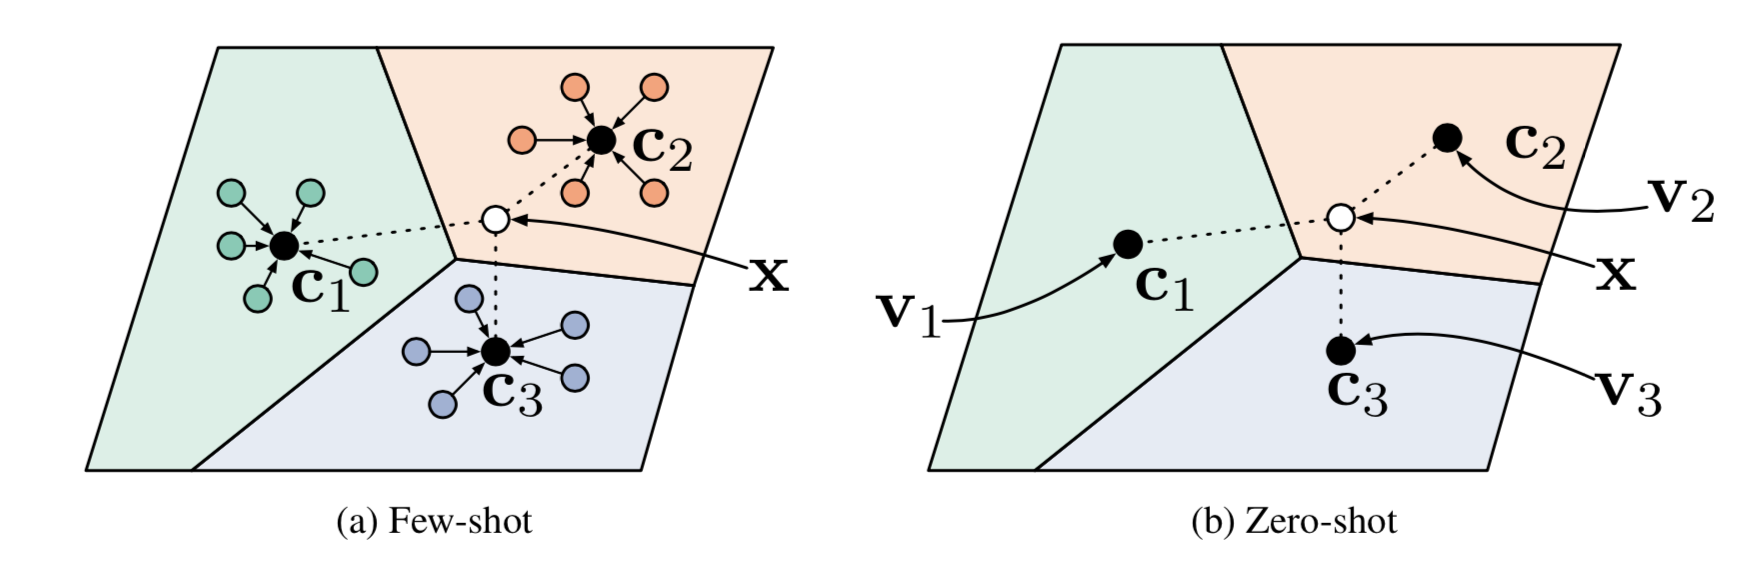
\includegraphics[width=0.8\textwidth]{background/prototypical-networks.png}
        \caption{Prototypical networks in the few-shot and zero-shot scenarios \cite{protonet}. \textbf{Left}: Few-shot prototypes $c_k$ are computed as the mean of embedded support examples for each class. \textbf{Right}: Zero-shot prototypes $c_k$ are produced by embedding class meta-data $v_k$. In either case, embedded query points are classified via a softmax over distances to class prototypes: \\ $p_{\phi}(y = k|x)$ $\alpha$ $e^{-d(f_{\phi}(x), c_k)}$.}
    \label{figure:background:prototypical}
\end{figure}

Prototypical Networks applies a compelling inductive bias in the form of class prototypes to achieve impressive few-shot performance. The key assumption is made is that there exists an embedding in which samples from each class cluster around a single prototypical representation which is simply the mean of the individual samples. This idea streamlines n-shot classification in the case of $n > 1$ as classification is simply performed by taking the label of the closest class prototype.

\begin{equation}
    c_k = \frac{1}{|S_k|} \sum_{(\mathbf{x}_i, y_i) \in S_k} f_{\phi}(\mathbf{x}_i)
\end{equation}
\captionof{figure}{Equation (1) from Prototypical Network calculating class prototypes. $S_k$ is the support set belonging to class $k$ and $f_{\phi}$ is the embedding function. \\}

Prototypical Networks are also amenable to zero-shot learning, as they allow to learn class prototypes directly from a high level description of a class such as labelled attributes or a natural language description. Afterwards it is possible to classify new images as a particular class without having seen an image of that class.

\subsection{DenseNet}

As our state of the art model we selected DenseNet because it can handle small datasets with low error rate\cite{pmlr-v80-pham18a}.

DenseNet \cite{densenet} works by concatenating the feature-maps of a convolutional block to the feature-maps of all the previous convolutional blocks and using this value as input for the next convolutional block. This way each convolutional block receives all the collective knowledge of the previous layers maintaining the global state of the network which can be accessed.

Convolutional networks construct informative features by fusion both spatial and chanel-wise information within local receptive fields at each layer. Squeeze and excitation blocks (SE block) \cite{Hu2017SqueezeandExcitationN} focus on the chanel-wise information used in the convolutional layers. SE blocks improve the quality of representations produced by the network by modeling the interdependency between channels to perform feature recalibration. SE blocks can be included in any model that uses convolutional layers to improve its performance at low computational cost. We added SE blocks to our DenseNet model to improve its performance.

\subsection{Data Augmentation}

Image data augmentation is a set of techniques that aim at artificially augmenting the amount of data that can be obtained from the images in the dataset. These techniques modify the images in the dataset  with a set of predefined operations to create new images that can be used to train a model.  In this manner, we can compensate  for the lack of  variability in a small dataset\cite{cubuk2019autoaugment}.
